\documentclass[margin=5mm]{standalone}
\usepackage{tikz}
\usetikzlibrary{matrix,calc}

\usepackage{amsfonts, 
			amssymb, 
			amsmath}

\DeclareMathAlphabet\mathbfcal{OMS}{cmsy}{b}{n}

\begin{document}
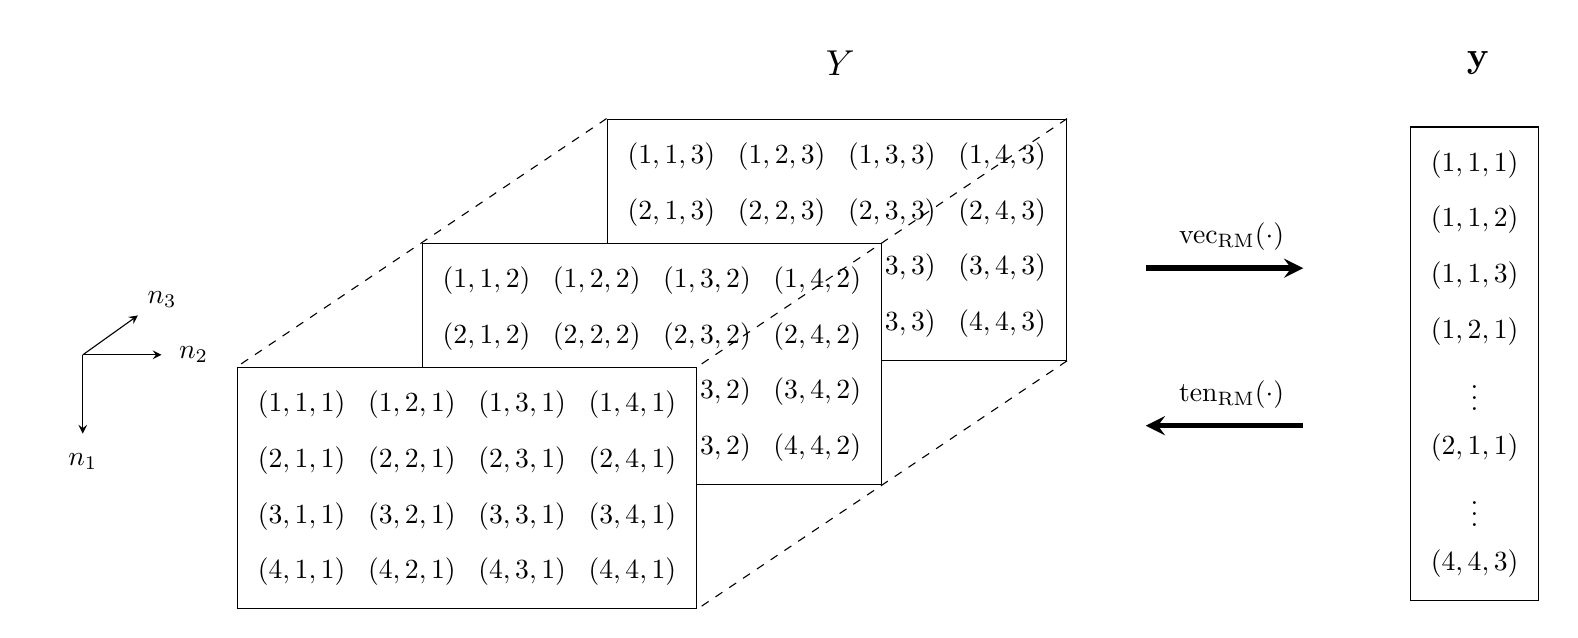
\begin{tikzpicture}[every node/.style={anchor=north east,fill=white,minimum width=1.4cm,minimum height=7mm}]

\node [below,opacity=0,text opacity=1] at (-12.5,-4) {$n_1$};
\node [right,opacity=0,text opacity=1] at (-11.8,-3.0) {$n_2$};
\node [right,opacity=0,text opacity=1] at (-12.2,-2.3) {$n_3$};

\draw [-stealth](-12.5,-3) -- (-12.5,-4);
\draw [-stealth](-12.5,-3) -- (-11.5,-3);
\draw [-stealth](-12.5,-3) -- (-11.8,-2.5);



\matrix (mA) [draw,matrix of math nodes]
{
(1,1,3) & (1,2,3) & (1,3,3) & (1,4,3) \\
(2,1,3) & (2,2,3) & (2,3,3) & (2,4,3) \\
(3,1,3) & (3,2,3) & (3,3,3) & (3,4,3) \\
(4,1,3) & (4,2,3) & (4,3,3) & (4,4,3) \\
};

\matrix (mB) [draw,matrix of math nodes] at ($(mA.south west)+(3.5,1.5)$)
{
(1,1,2) & (1,2,2) & (1,3,2) & (1,4,2) \\
(2,1,2) & (2,2,2) & (2,3,2) & (2,4,2) \\
(3,1,2) & (3,2,2) & (3,3,2) & (3,4,2) \\
(4,1,2) & (4,2,2) & (4,3,2) & (4,4,2) \\
};

\matrix (mC) [draw,matrix of math nodes] at ($(mB.south west)+(3.5,1.5)$)
{
(1,1,1) & (1,2,1) & (1,3,1) & (1,4,1) \\
(2,1,1) & (2,2,1) & (2,3,1) & (2,4,1) \\
(3,1,1) & (3,2,1) & (3,3,1) & (3,4,1) \\
(4,1,1) & (4,2,1) & (4,3,1) & (4,4,1) \\
};

\draw[dashed](mA.north east)--(mC.north east);
\draw[dashed](mA.north west)--(mC.north west);
\draw[dashed](mA.south east)--(mC.south east);

\node [right,opacity=0,text opacity=1] at (1.3,-1.5) {$\text{vec}_{\text{RM}}(\cdot)$};
\draw [-stealth, line width=2pt](1,-1.9) -- (3,-1.9);

\node [right,opacity=0,text opacity=1] at (1.3,-3.5) {$\text{ten}_{\text{RM}}(\cdot)$};
\draw [stealth-, line width=2pt](1,-3.9) -- (3,-3.9);

\node [right,opacity=0,text opacity=1,scale=1.3] at (4.3,0.7) {$\mathbf{y}$};
\node [right,opacity=0,text opacity=1,scale=1.3] at (-3.8,0.7) {$\mathbfcal{Y}$};



\matrix (mD) [draw, matrix of math nodes] at (6, -0.1)
{
(1,1,1) \\
(1,1,2) \\
(1,1,3) \\
(1,2,1) \\
\vdots \\
(2,1,1) \\
\vdots \\
(4,4,3)  \\
};

\end{tikzpicture}
\end{document}